\section{Pipeline}

Surface reconstruction from measurement data is often a step by step process:

\begin{itemize}
\item Scanning and scan alignment produce a set of points
      or points with normals. Alignment is not yet
      covered by \cgal.
\item Outlier removal for reconstruction methods which
      are not resilient to outliers.
\item Simplification to reduce the number of input points.
\item Smoothing to reduce noise in the input data.
\item Normal estimation and orientation when the normals
      are not already provided by the acquisition device.
\item Surface reconstruction.
\end{itemize}

This component provides algorithms for all steps listed above, except alignment.
A demo running on Windows is currently provided, and we will elaborate soon upon a new point set demo based on QT4 and QGlViewer.

% Insert image pipeline.jpg/eps
\begin{center}
    \label{Surface_reconstruction_3-fig-pipeline}
    % Image
    \begin{ccTexOnly}
        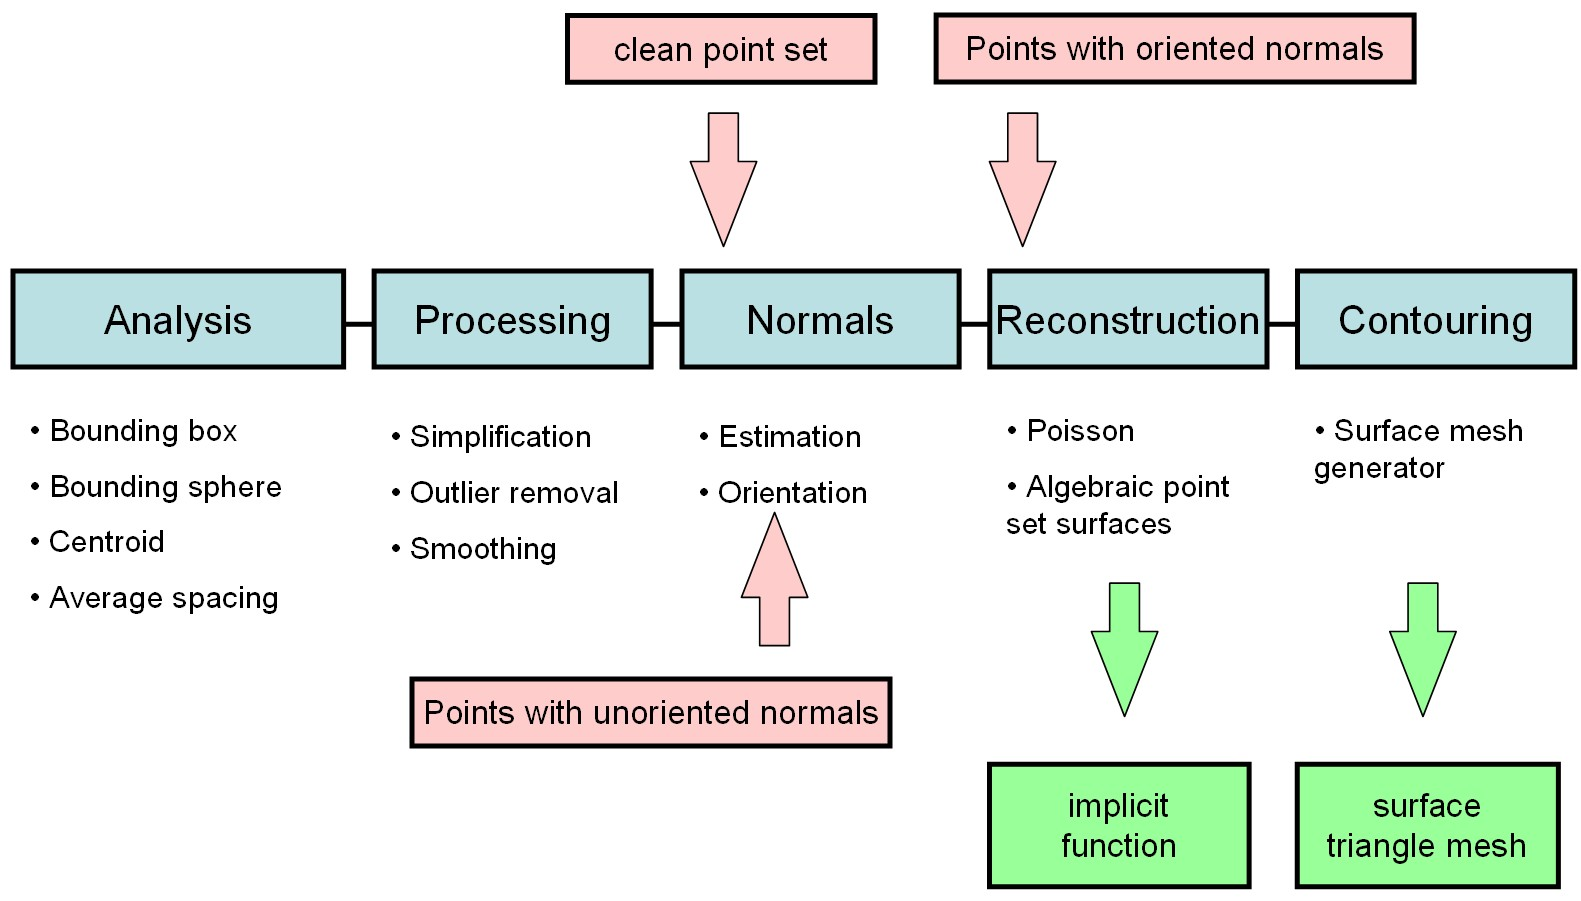
\includegraphics[width=1.0\textwidth]{Surface_reconstruction_3/pipeline} % omit .eps suffix
    \end{ccTexOnly}
    \begin{ccHtmlOnly}
        <img width="70%" border=0 src="./pipeline.jpg"><P>
    \end{ccHtmlOnly}
    % Title
    \begin{figure}[h]
        \caption{Surface reconstruction pipeline.}
    \end{figure}
\end{center}


\subsection{Input}

Functions and classes of this component expect as input and output parameters range iterators over:

\begin{itemize}
\item 3D points
\item Normals (orientable 3D vectors)
\item 3D points with unoriented normals
\item 3D points with oriented normals
\end{itemize}

We provide several models of points and normals concepts, with different speed/space trade-offs:

\begin{itemize}
\item \ccRefIdfierPage{CGAL::Point_3<GeomTraits>} \\
\cgal\ 3D position.
\item \ccRefIdfierPage{CGAL::Vector_3<GeomTraits>} \\
\cgal\ 3D vector.
\item \ccRefIdfierPage{CGAL::Lightweight_vector_3<GeomTraits>} \\
3D vector allocated only if not (0,0,0).
\item \ccRefIdfierPage{CGAL::Orientable_normal_3<GeomTraits>} \\
Normal (oriented or not).
Inherits from \ccc{Vector_3<GeomTraits>} and contains an "is normal oriented?" flag.
\item \ccRefIdfierPage{CGAL::Point_with_normal_3<GeomTraits, Normal_3>} \\
3D position + normal.
\end{itemize}

In addition, we provide convenient functions to read point sets from standard file formats:

\begin{itemize}
\item XYZ
\item OFF
\end{itemize}

\ccRefIdfierPage{CGAL::surface_reconstruction_read_xyz}  \\
\ccRefIdfierPage{CGAL::surface_reconstruction_read_off_point_cloud}  \\

Example:

\ccIncludeExampleCode{Surface_reconstruction_3/surface_reconstruction_read_write_xyz_example.cpp}


\subsection{Analysis}

The purpose of the analysis stage is to measure common statistics and bounding volumes over the input points
so as to automatically determine parameters for subsequent stages downstream along the pipeline:
\begin{itemize}
  \item Point set barycenter, bounding box,
        bounding sphere (provided by other \cgal\ components).
  \item Average spacing to the $k$ nearest neighbors.
\end{itemize}

\ccc{CGAL::average_spacing_3()} computes the average spacing of all input points to their $k$ nearest neighbors.

\ccRefIdfierPage{CGAL::centroid}  \\
\ccRefIdfierPage{CGAL::bounding_box}  \\
\ccRefIdfierPage{CGAL::bounding_sphere}  \\
\ccRefIdfierPage{CGAL::average_spacing_3}  \\

Example:

\ccIncludeExampleCode{Surface_reconstruction_3/average_spacing_example.cpp}


\subsection{Processing}

Processing refers to all algorithms which alter the input points so as to remove outliers, reduce noise by smoothing, and simplify.

\subsubsection{Outlier Removal}

Function \ccc{CGAL::outlier_removal_3()} deletes a user-specified fraction of outliers from the input point set.
More specifically, it sorts the input points in increasing order of average squared distances to the $k$ nearest neighbors
and deletes the points with largest value.

\emph{Note to the reviewers: we will add a function in the analysis section which displays in the console the distribution of such average squared distance so as to help the user picking an appropriate fraction value.}

\ccRefIdfierPage{CGAL::outlier_removal_3}  \\

% % Insert image outlier_removal.jpg/eps
% \begin{center}
%     \label{Surface_reconstruction_3-fig-outlier_removal}
%     % Image
%     \begin{ccTexOnly}
%         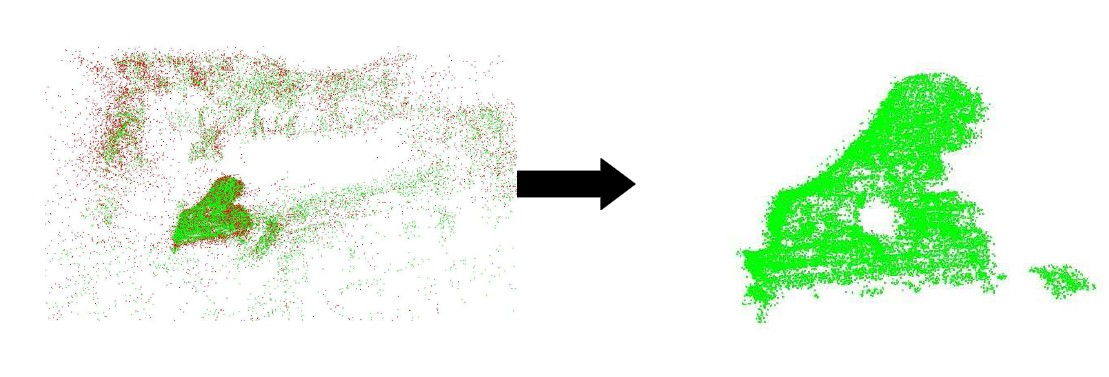
\includegraphics[width=0.9\textwidth]{Surface_reconstruction_3/outlier_removal} % omit .eps suffix
%     \end{ccTexOnly}
%     \begin{ccHtmlOnly}
%         <img width="90%" border=0 src="./outlier_removal.jpg"><P>
%     \end{ccHtmlOnly}
%     % Title
%     \begin{figure}[h]
%         \caption{Outlier removal}
%     \end{figure}
% \end{center}

Example:

\ccIncludeExampleCode{Surface_reconstruction_3/outlier_removal_example.cpp}


\subsubsection{Simplification}

Two functions are provided to simplify the input point set.

\ccc{CGAL::merge_simplification_3()} iteratively merges pairs of points which are epsilon-closed.

\ccc{CGAL::random_simplification_3()} randomly deletes a user-specified fraction of points from the input point set.

\ccRefIdfierPage{CGAL::merge_simplification_3}  \\
\ccRefIdfierPage{CGAL::random_simplification_3}  \\

% Insert image merge_simplification.jpg/eps
\begin{center}
    \label{Surface_reconstruction_3-fig-merge_simplification}
    % Image
    \begin{ccTexOnly}
        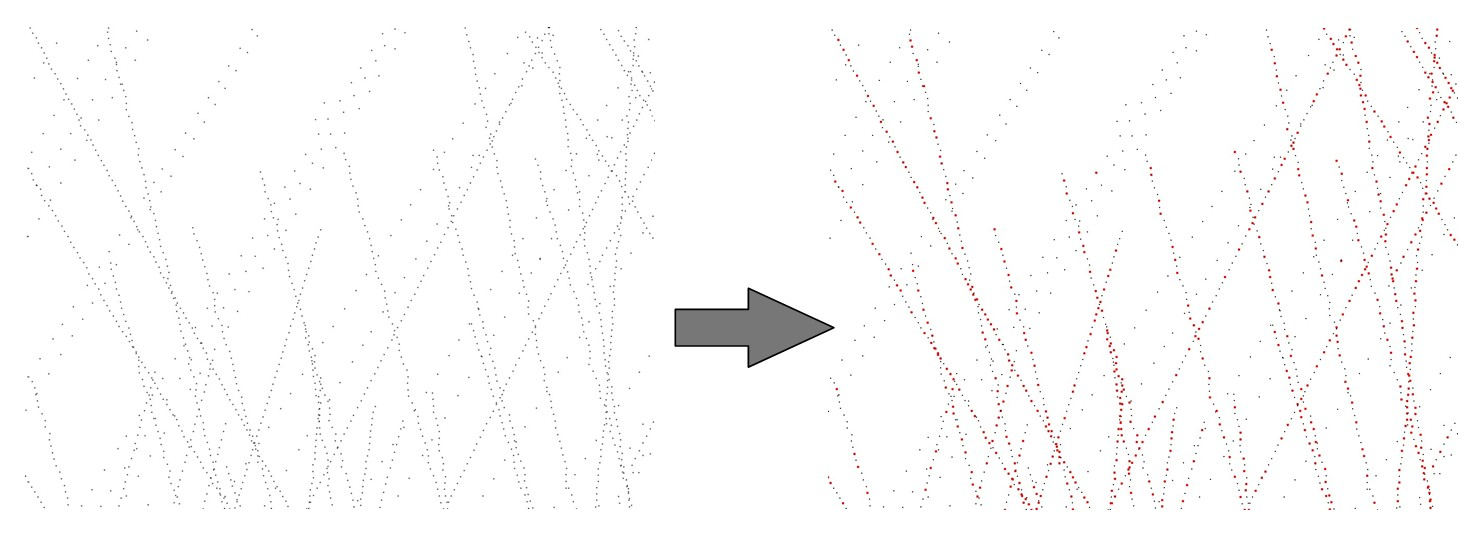
\includegraphics[width=0.7\textwidth]{Surface_reconstruction_3/merge_simplification} % omit .eps suffix
    \end{ccTexOnly}
    \begin{ccHtmlOnly}
        <img width="100%" border=0 src="../Surface_reconstruction_3/merge_simplification.jpg"><P>
    \end{ccHtmlOnly}
    % Title
    \begin{figure}[h]
        \caption{Point set simplification by merging.
                 Left: input point set.
                 Right: removed points are depicted in red.}
    \end{figure}
\end{center}

Example:

\ccIncludeExampleCode{Surface_reconstruction_3/random_simplification_example.cpp}


\subsubsection{Smoothing}

Function \ccRefIdfierPage{CGAL::jet_smoothing_3} smooths the input point set by projecting each point
onto a smooth parametric surface patch (so-called jet surface) fitted over the $k$ nearest neighbors. \\

% % Insert image jet_smoothing.jpg/eps
% \begin{center}
%     \label{Surface_reconstruction_3-fig-jet_smoothing}
%     % Image
%     \begin{ccTexOnly}
%         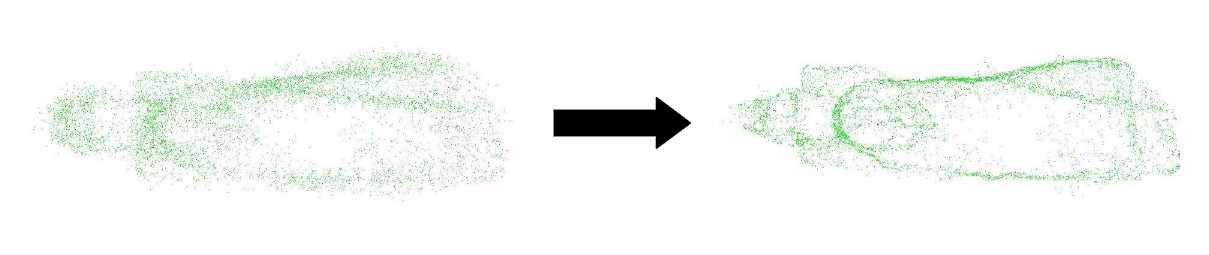
\includegraphics[width=1.0\textwidth]{Surface_reconstruction_3/jet_smoothing} % omit .eps suffix
%     \end{ccTexOnly}
%     \begin{ccHtmlOnly}
%         <img width="100%" border=0 src="./jet_smoothing.jpg"><P>
%     \end{ccHtmlOnly}
%     % Title
%     \begin{figure}[h]
%         \caption{Point set smoothing}
%     \end{figure}
% \end{center}

Example:

\ccIncludeExampleCode{Surface_reconstruction_3/jet_smoothing_example.cpp}


\subsubsection{Normal Estimation}

Two functions are provided to estimate the normal direction of the inferred surface at each point from the input point set.
In both cases, the result is an unoriented normal vector for each input point.

Function \ccc{CGAL::jet_normal_estimation()} estimates the normal direction at each point from the set
by fitting a jet surface over its $k$ nearest neighbors. The default jet is a quadric surface.

Function \ccc{CGAL::pca_normal_estimation()} estimates hte normal direction at each point from the set
by linear least squares fitting of a plane over its $k$ nearest neighbors.

\ccRefIdfierPage{CGAL::pca_normal_estimation}  \\
\ccRefIdfierPage{CGAL::jet_normal_estimation}  \\

% % Insert image pca_normal_estimation.jpg/eps
% \begin{center}
%     \label{Surface_reconstruction_3-fig-pca_normal_estimation}
%     % Image
%     \begin{ccTexOnly}
%         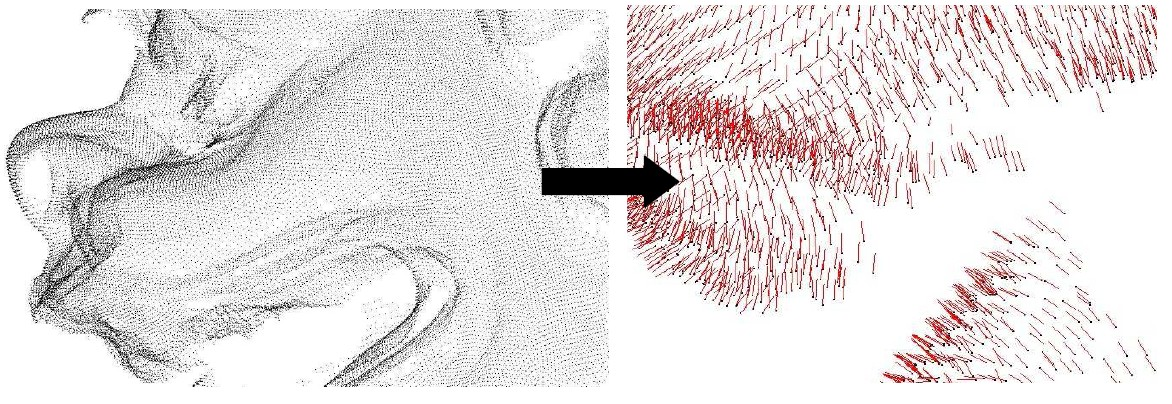
\includegraphics[width=0.9\textwidth]{Surface_reconstruction_3/pca_normal_estimation} % omit .eps suffix
%     \end{ccTexOnly}
%     \begin{ccHtmlOnly}
%         <img width="90%" border=0 src="./pca_normal_estimation.jpg"><P>
%     \end{ccHtmlOnly}
%     % Title
%     \begin{figure}[h]
%         \caption{Normal estimation by Principal Components Analysis}
%     \end{figure}
% \end{center}

Example:

\ccIncludeExampleCode{Surface_reconstruction_3/pca_normal_estimation_example.cpp}


\subsubsection{Normal Orientation}

Function \ccc{CGAL::mst_normal_orientation()} orients the normals of a set of points with (unoriented) normals
using the method described by Hoppe et al. in {\em Surface reconstruction from unorganized points} \cite{cgal:hddms-srup-92}.
More specifically, this method constructs a Riemannian graph over the input points and
propagates a seed normal orientation within a minimum spanning tree computed over the graph with the Boost graph library.
The result is an oriented normal vector for each input point/normal.

\ccRefIdfierPage{CGAL::mst_normal_orientation}  \\

% Insert image mst_normal_orientation.jpg/eps
\begin{center}
    \label{Surface_reconstruction_3-fig-mst_normal_orientation}
    % Image
    \begin{ccTexOnly}
        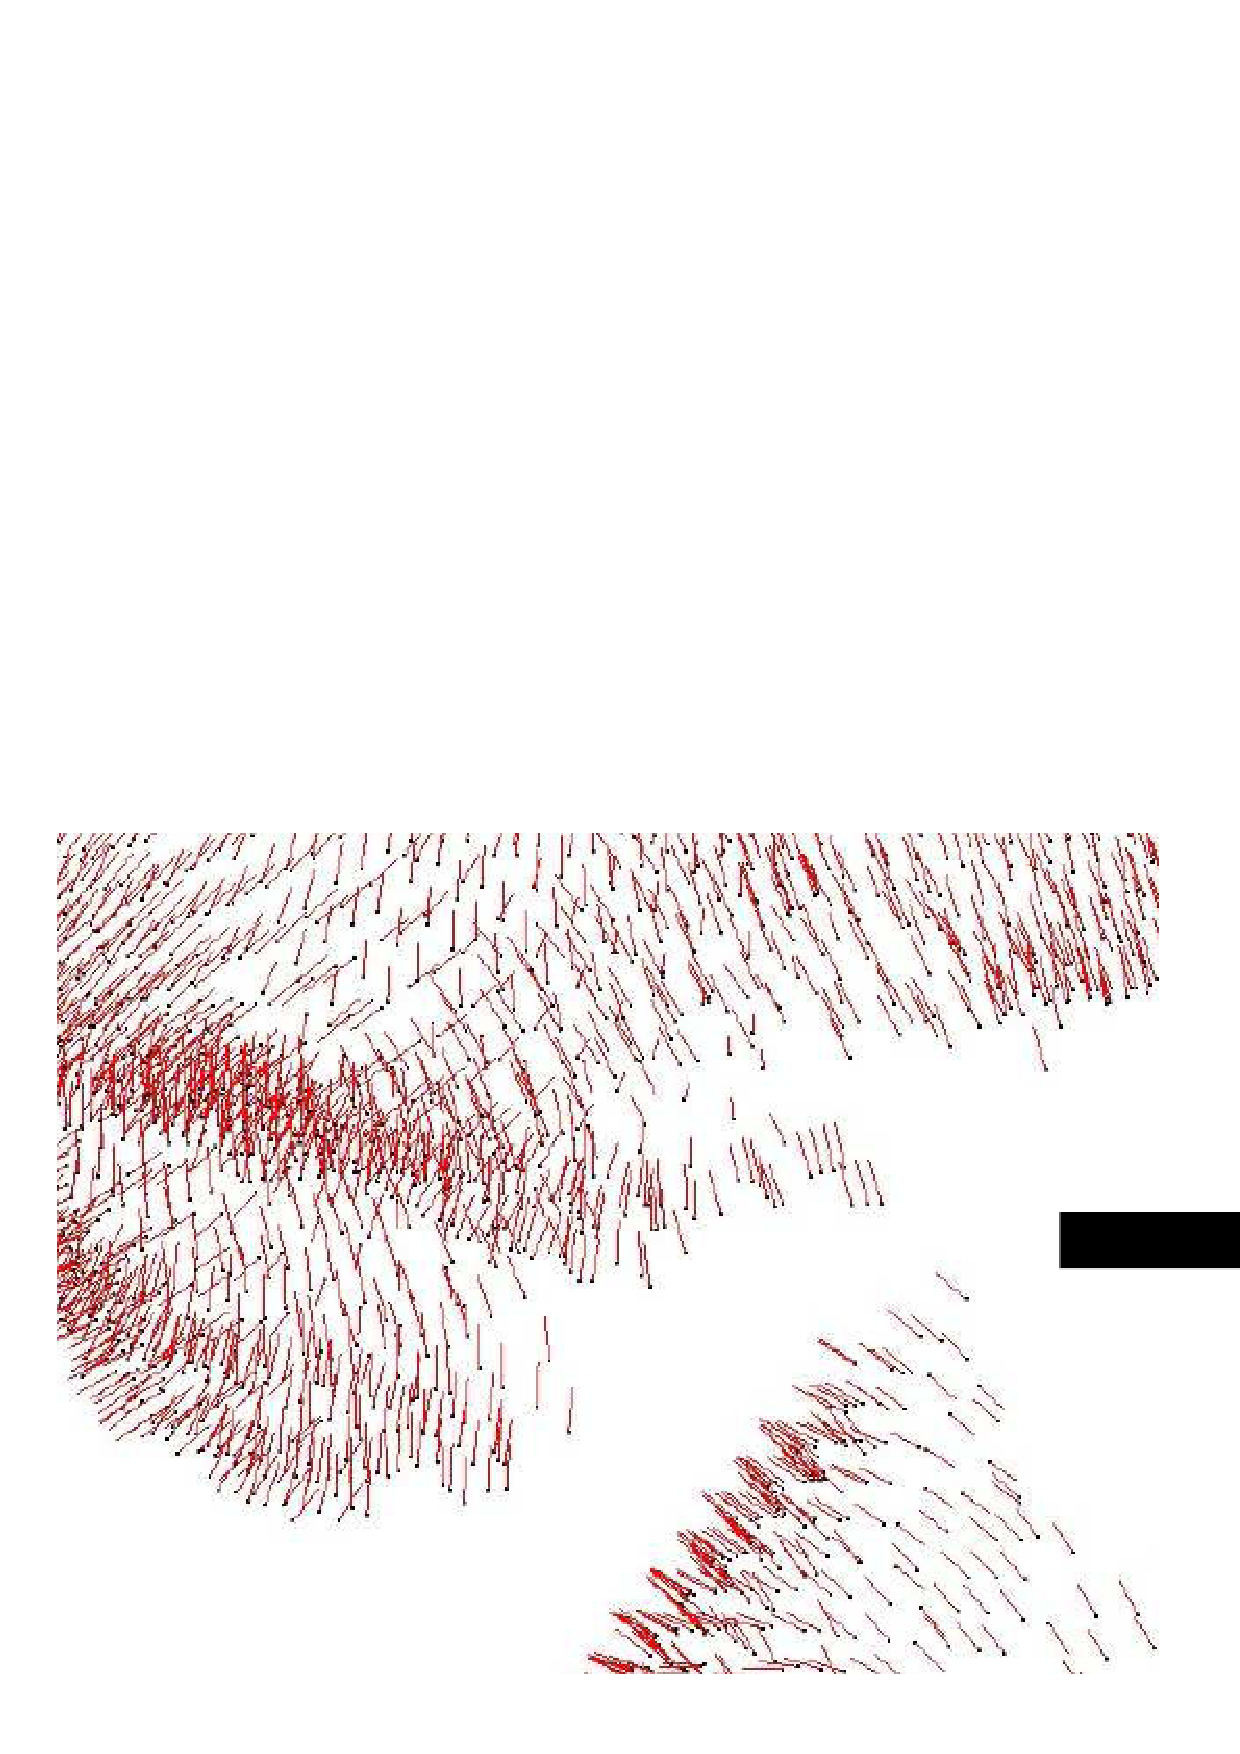
\includegraphics[width=0.9\textwidth]{Surface_reconstruction_3/mst_normal_orientation} % omit .eps suffix
    \end{ccTexOnly}
    \begin{ccHtmlOnly}
        <img width="90%" border=0 src="./mst_normal_orientation.jpg"><P>
    \end{ccHtmlOnly}
    % Title
    \begin{figure}[h]
        \caption{Normal orientation}
    \end{figure}
\end{center}

Example: see \ccc{pca_normal_estimation_example.cpp} example above.

\subsection{Surface Reconstruction}

The two surface reconstruction methods fall into the category of the implicit surface reconstruction approaches in the sense that they both compute a scalar function whose iso-surface approximates the input oriented points.
\begin{itemize}
\item Delaunay-based Poisson reconstruction inspired
      from \cite{Kazhdan06}. This method solves for
      an approximate indicator function of the inferred
      solid. The solving stage must be done once for all
      before iso-contouring. % refer to basics?
\item Algebraic point set surfaces \cite{Guennebaud07}.
      This method falls into the category of so-called
      point set surfaces, where the approximate
      signed distance function to the inferred surface
      can be evaluated at any query point and on the fly
      during iso-contouring.
\end{itemize}

\ccRefIdfierPage{CGAL::Poisson_reconstruction_function<GeomTraits, ReconstructionTriangulation_3>}  \\
\ccRefIdfierPage{CGAL::APSS_reconstruction_function<GeomTraits>}  \\

% Insert image APSS.jpg/eps
\begin{center}
    \label{Surface_reconstruction_3-fig-APSS}
    % Image
    \begin{ccTexOnly}
        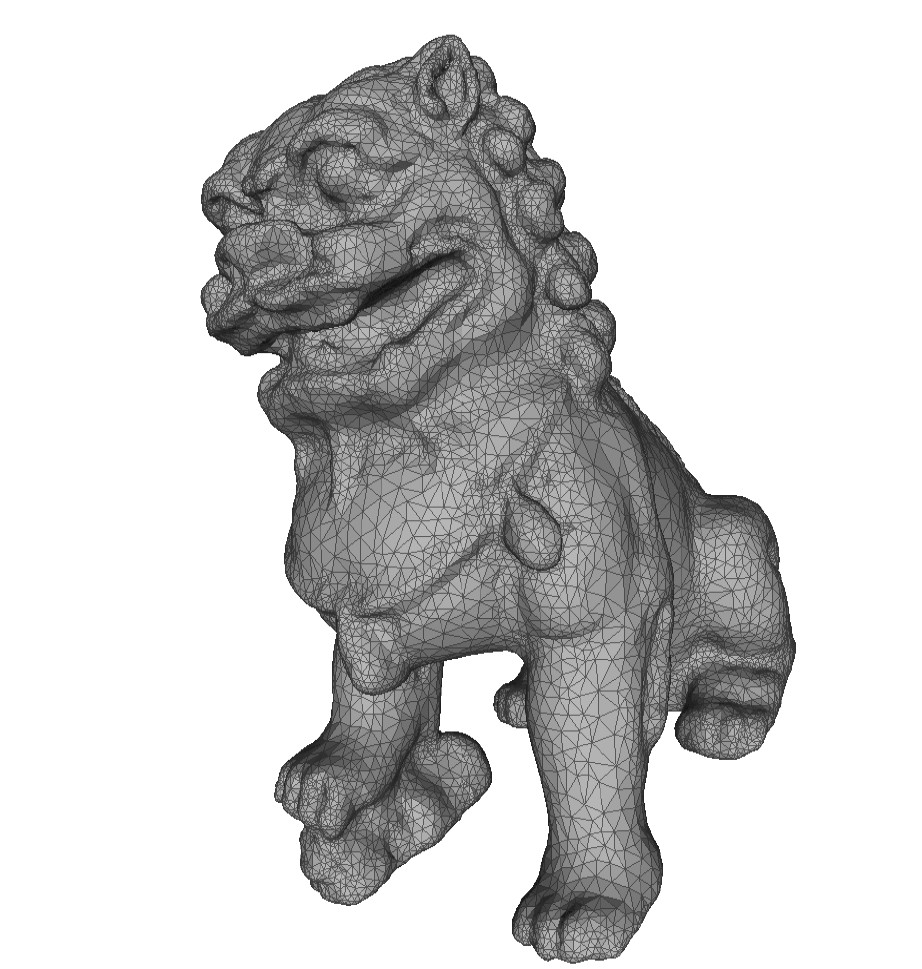
\includegraphics[width=0.5\textwidth]{Surface_reconstruction_3/APSS} % omit .eps suffix
    \end{ccTexOnly}
    \begin{ccHtmlOnly}
        <img width="50%" border=0 src="./APSS.jpg"><P>
    \end{ccHtmlOnly}
    % Title
    \begin{figure}[h]
        \caption{APSS reconstruction.
        Left: points with oriented normals.
        Right: reconstructed surface mesh.}
        % later in the middle: computed function
    \end{figure}
\end{center}


The computed ``implicit'' functions can be iso-contoured to reconstruct a surface by using the \cgal\ surface mesh generator~\cite{cgal:ry-gsddrm-06,cgal:bo-pgsms-05}.

\ccRefIdfierPage{CGAL::make_surface_mesh}  \\

The parameter \ccc{Tag} affects the behavior of \ccc{make_surface_mesh()}: \\
- \ccc{Manifold_tag}: the output mesh is guaranteed to be a  manifold surface without boundary.\\
- \ccc{Manifold_with_boundary_tag}: the output mesh is guaranteed to be manifold and may have boundaries.\\
- \ccc{Non_manifold_tag}: the output mesh has no guarantee and hence is outputted as a polygon soup.

Example:
See \ccc{poisson_reconstruction_example.cpp} example above.


\subsection{Output}

\subsubsection{Point Set Output}

The output of the processing stage is a point set with normals.
For convenience, we provide functions to write point sets to standard file formats:
\begin{itemize}
\item XYZ
\item OFF
\end{itemize}

\ccRefIdfierPage{CGAL::surface_reconstruction_write_off_point_cloud}  \\
\ccRefIdfierPage{CGAL::surface_reconstruction_write_xyz}  \\

Example:

See \ccc{surface_reconstruction_read_write_xyz_example.cpp} example above.


\subsubsection{Surface Output}

The surface reconstructed by \ccc{make_surface_mesh()}
is required to be a model of the concept
\ccc{SurfaceMeshComplex_2InTriangulation_3},
a data structure devised to represent a two dimensional
complex embedded into a three dimensional triangulation.\\

\ccc{SurfaceMeshComplex_2InTriangulation_3} defines the methods to traverse the reconstructed surface.

As examples, we provide functions to:

\begin{itemize}
\item Write the reconstructed surface mesh to the
      OFF file format.
\item Convert the reconstructed surface mesh to a
      polygon soup.
\end{itemize}

\ccRefIdfierPage{CGAL::output_surface_facets_to_off}  \\
\ccRefIdfierPage{CGAL::surface_reconstruction_output_surface_facets}  \\

Example:

See \ccc{poisson_reconstruction_example.cpp} example above.






